\section{Testing e performance}

% Esporre lo stato di funzionamento effettivo del sistema progettato ad elaborato concluso.
% Per ciascuna delle funzionalità salienti devono essere tabellate e discusse le performance riscontrate mediante opportuni test eseguiti in fase di validazione del progetto.

% I tempi di esecuzione/comunicazione devono essere accompagnati dalle caratteristiche dell'hardware sul quale è eseguito il software.

% Qualora l'elaborato includa algoritmi innovativi, indicarne la complessità computazionale (avendo cura di esporre lo pseudo codice nella sezione implementazione).

% Vincoli circa la lunghezza della sezione (escluse didascalie, tabelle, testo nelle immagini, schemi):
% Numero minimo di battute per 2 componenti: 2500
% Numero massimo di battute per 2 componenti: 4500

\subsection{Testing durante lo sviluppo}

Per quanto riguarda i piani di test, abbiamo deciso di adottare un approccio manuale:
non potendo contare su particolari framework dedicati, abbiamo realizzato la maggior parte delle prove manualmente.

\subsubsection[Backend]{Backend (Fog \& Cloud)}

Per quanto riguarda entrambi i backend, le API REST sono state testate manualmente tramite Postman\footnote{\url{https://www.getpostman.com/}}, strumento specifico per questo tipo di operazioni:
ogni volta che una nuova API veniva aggiunta al sistema, questa veniva
testata con tale strumento per verificare non solo che il server la esponesse correttamente,
ma anche che la Business Logic a essa collegata corrispondesse a quanto pensato in fase di progettazione.

Anche la comunicazione con il database, realizzata dopo le API, è stata testa tramite Postman, verificando dalla Firebase Cloud Console che le pubblicazioni sul DB fossero corrette.

Infine la comunicazione con MQTT, realizzata anch'essa dopo le API, è stata testata pubblicando tramite MQTT Explorer\footnote{\url{http://mqtt-explorer.com/}} rilevazioni fittizie e verificando che l'esecuzione andasse a buon fine tramite API e log.

\subsubsection[Frontend]{Frontend (Fog \& Cloud)}

Il codice relativo al frontend web è stato anch'esso testato manualmente, sia tramite server \emph{mock} quando le API non erano ancora pronte, sia con le API reali quando disponibili.

\subsubsection{Sensori IoT}

Il codice eseguito su ESP8266 è stato anch'esso realizzato con approccio incrementale, verificando prima tramite comunicazione seriale che le rilevazioni fossero corrette, e poi via MQTT Explorer che venissero pubblicate come da aspettative.

\subsection{Testing del sistema finale}

Una volta giunti a termine dello sviluppo, si è reso necessario testare il sistema in ogni sua funzionalità.

Il sistema è stato dunque posizionato in una stanza della Biblioteca Centrale Roberto Ruffilli del Campus di Forlì per alcune ore, monitorando le rilevazioni tramite entrambe le interfacce web.

\subsubsection{Hardware utilizzato}

Per quanto riguarda l'hardware impiegato per il testing, sono state utilizzate le seguenti risorse:

\begin{itemize}
  \item
    \strong{Raspberry Pi 3 Model B} come Fog server;
    un ricevitore USB WiFi è stato collegato per poter gestire con stabilità sia la connessione \emph{upstream} ad AlmaWiFi che l'hotspot per il sensore.
    Il dispositivo è stato alimentato tramite una batteria al litio da 3700mAh.
  \item \strong{NodeMCU ESP8266} come sensore IoT, alimentato tramite un powerbank da 3350mAh.
\end{itemize}

\begin{figure}[H]
  \centering
  \begin{subfigure}[htbp]{0.45\textwidth}
    \centering
    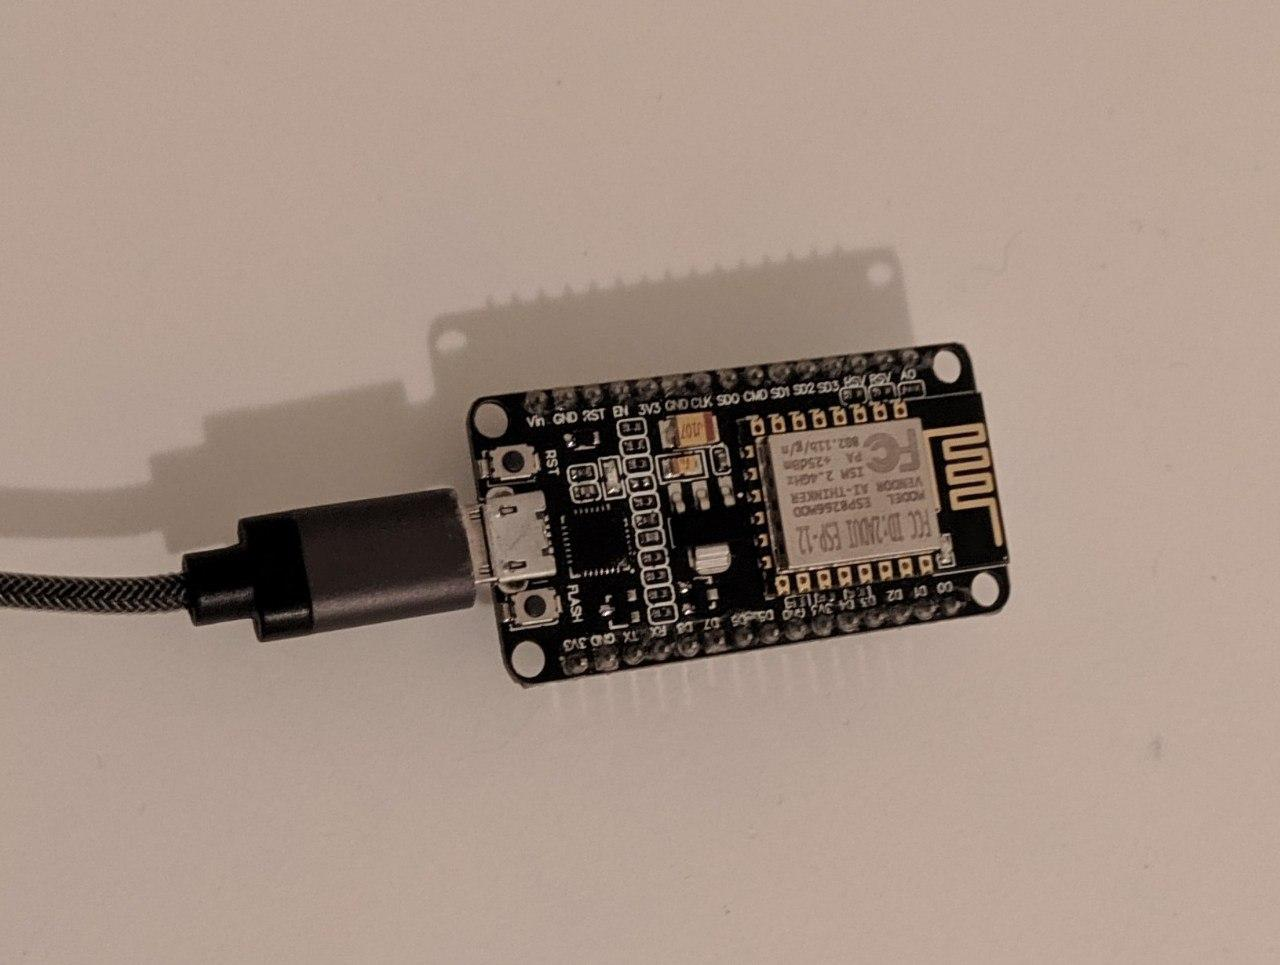
\includegraphics[width=\textwidth]{res/fig/esp.jpg}%
    \label{subfig:esp}
  \end{subfigure}
  \hfill
  \begin{subfigure}[htbp]{0.45\textwidth}
    \centering
    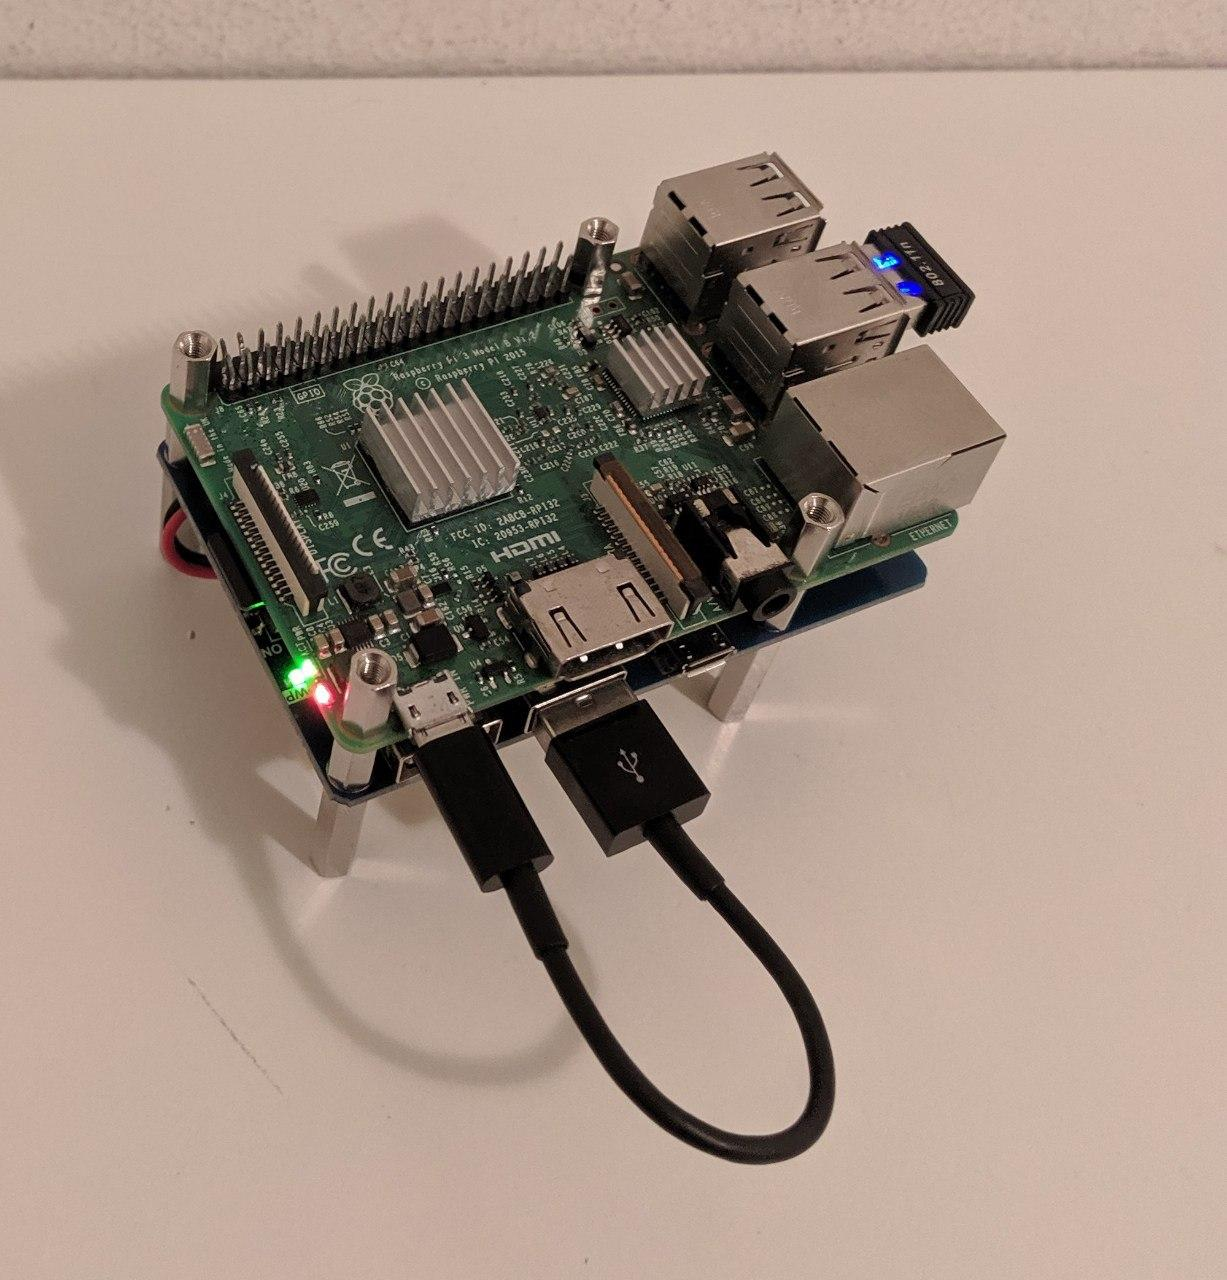
\includegraphics[width=\textwidth]{res/fig/rpi.jpg}%
    \label{subfig:raspi}
  \end{subfigure}
  \caption{Fotografie del prototipo di sistema}%
  \label{fig:hw}
\end{figure}

\subsubsection{Performance ottenute}

In questa sezione è presente una breve trattazione delle perfomance riscontrate durante il testing delle principali feature del prototipo finale:

\begin{description}
  \item[Avvio del sistema]
    Considerando i differenti sistemi:
    \begin{itemize}
      \item Il Raspberry Pi impiega generalmente circa due minuti ad avviarsi e il broker MQTT viene messo in esecuzione in pochi secondi.
      \item Il container Docker che mette in esecuzione il jar generalmente si avvia in una decina di secondi al massimo.
      \item Il sensore su ESP8266 si avvia in pochi secondi.
    \end{itemize}
  \item[Scansione delle frequenze]
    L'ESP8266 impiega in media circa 5 minuti per effettuare la scansione di tutte le 14 frequenze del WiFi supportate.
  \item[Pubblicazione su MQTT]
    L'ESP8266 impiega 5--10 secondi a collegarsi alla rete WiFi ed effettuare la pubblicazione.
  \item[Gestione delle API]
    Il Raspberry Pi e il Cloud impiegano tempi molto simili per gestire le singole chiamate API\@:
    in media, sono necessari 5--10 secondi per ottenere una risposta se è coinvolto il database, altrimenti anche meno di 5 secondi.
\end{description}
